\chapter{System Diagram}
\begin{figure}[h]
\begin{center}
  % Requires \usepackage{graphicx}
  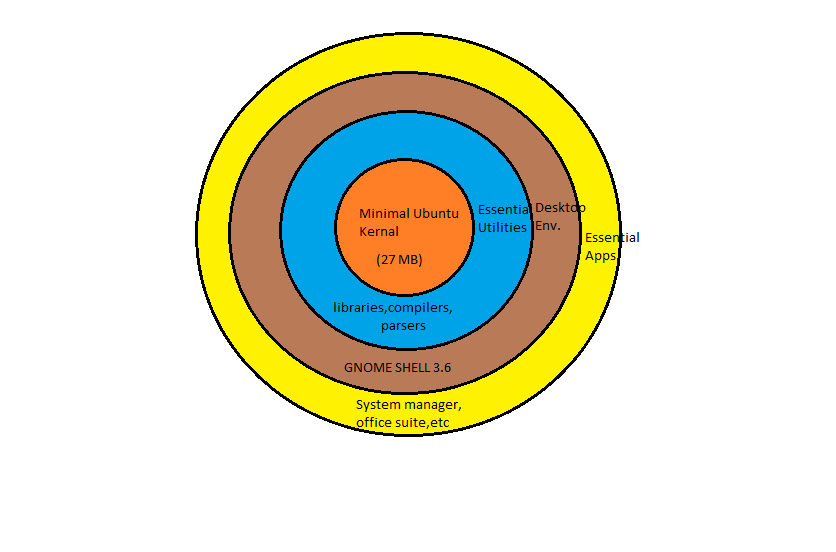
\includegraphics [scale=0.8] {core.png}
  \caption[System Ovierview]{Layered diagram of System}
\end{center}
\end{figure}
\begin{figure}[h]
\begin{center}
  % Requires \usepackage{graphicx}
  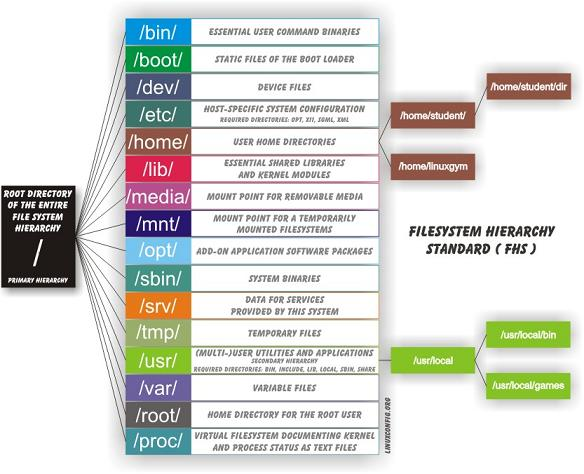
\includegraphics [scale=0.55] {dir.jpg}
  \caption[FIle system Diagram]{Linux File directories diagram}
\end{center}
\end{figure}

\chapter{Application Development}
We have developed some basic utilites that are going to enhance operating system experience.

\section{UTILITIES}
\begin{enumerate}

\item Auto ON Utility:\\
This application is developed with the aim of booting up PC at given time from shut down. This software is developed for Linux systems not for windows.
\begin{figure}[h]
\begin{center}
  % Requires \usepackage{graphicx}
  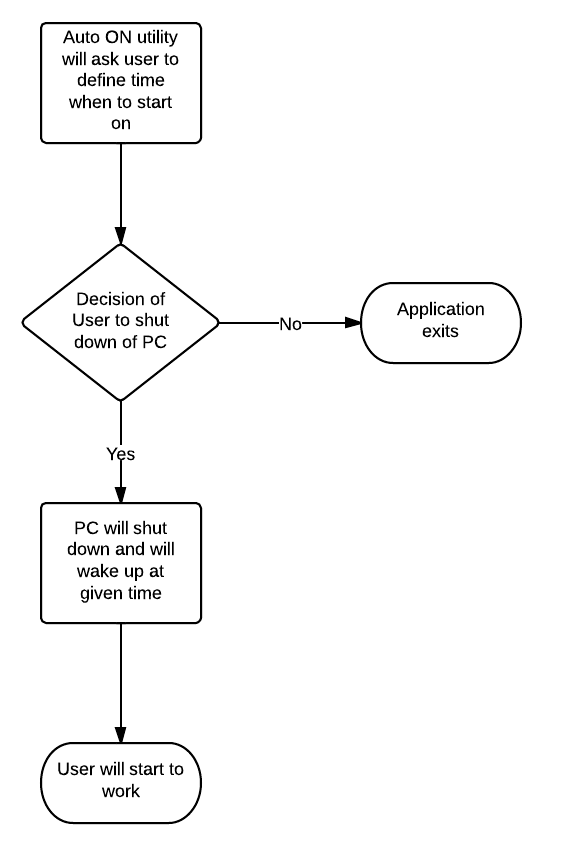
\includegraphics [scale=0.8] {aoutil.png}
  \caption[Auto ON Utility]{Auto ON Utility Flowchart}
\end{center}
\end{figure}

\item	LAMP(Front end)\\
This application is developed with the aim to handle LAMP Services(Apache, MySQL and PHP Services installed inside Linux system)

\item Repocloner\\
Repocloner is an application to make local apt repository for intranet based servers.
This application is for server side which has linux installed.
\item	Multidoc Converter\\
This application is developed with aim to convert multiple document formats between each other. 
\end{enumerate}

\section{Gujarati Dictionary}
\subsection {Purpose}
	This dictionary is general dictionary that will provide meaning of given English words into gujarati meaning.
	Dictionary is going to develop for OpenGujarat as well as this dictionary can be ported or installed in other system.
\subsection{Current Alternative Application}
	There is no dictionary (English to Gujarati) available for any linux(debian or RPM package management system) operating system till now. 
	This is our first time development in this space.

\subsection{Porting System}
We will try to port this dictionary on multiple platform in short time.
We have short time so we will try to use other third party application to port our dictionary in desired system.
Our dictionary can be insalled on Windows,Mac OS X,Android and Linux system.
\subsection{Component of Dictionary Development}
\subsubsection{Dictionary Front End}
	Dictionary front end means Dicitonary look up program. The application that gives interface between database and user to manipulate information in easy way.

\begin{itemize}
\item LINUX :\\
STAR DICT (APPLICATION)  or GOLDEN DICT(APPLICATION):\\
This front end application is available on Ubuntu repository. You can install via following commands.

\item	ANDROID:\\
Golden Dict(Application):\\
This front end application can be downloaded from Google play store.(Link)

\end{itemize}	
	\subsection{Dictionary back end}
Dictionary back end means the database that includes English words and meaning of that words in Gujarati.
	Database is provided by GujaratiLexicon.com.
	This database contains around 52,000 words.
